% this file is called up by thesis.tex
% content in this file will be fed into the main document

\chapter{Evaluation}\label{chap:evaluation} % top level followed by section, subsection
In this chapter we will present the results found by our framework, and some challenges we encountered during the gathering of the results.

\section{Setup}
We ran the framework on Ubuntu 18.04 LTS inside a QEMU virtual environment with 62 CPU cores on an AMD ThreadRipper \todo{Ask for model name} processor with 64GB of RAM on which we also compiled the binaries and collected the traces.

We compiled every binary 5 times, twice with the modified Angora compiler, namely one for the fast instrumentation and one with the track instrumentation, once with the SymCC compiler, once with the Fuzz Checker compiler to create the Oracle and once with the static analysis pass.

We collected the traces by letting the fuzzer run for 8 hours on all 62 cores. Then we give every strategy a maximum of 15 seconds of execution time per condition in a trace. For the ConcolicStrategy, we give it 13 seconds to calculate the possible executions and the last 2 seconds can be used to try the generated inputs. The execution time of the target binary is included in the execution time of a strategy, since the total time is the time one is interested in when trying to implement the most efficient strategy.

\section{Challenges}
During our tests we noticed that the \texttt{xmlwf} binary did not generate any test cases for the ConcolicStrategy. After inspection with \texttt{ltrace} we noticed that it did made library calls to the \texttt{SymCC} library, so we decided to mark this strategy for this binary as failed.

In order to compile the \texttt{libpng} library used for the \texttt{gif2png} program, the \texttt{zlib} library was required, so we also compiled and linked this library to \texttt{libpng} using our instrumentation. 

For the \texttt{tiff2pdf} binary, we got a lot of warnings from Angora during the initial fuzzing that some conditions were inconsistent between the track and the fast instrumentation runs. These programs were also not tested in the Angora paper. However, there were still track files outputted an new conditions found. The conditions which were inconsistent were marked as such and discarded during our runs. When we started analysing these traces, we found that the there was not a single condition flipped for this binary. After a inspection in \texttt{gdb} we found that the context ids had changed between the collected tracks and the inserted context ids of our own instrumentation. It is unclear why this happened for only this binary, but it could be that something already went wrong during the collection of the traces. To be completely sure that we accidentally compiled the two versions in different environments, we cloned the source repository after every compilation, to make sure we were in the exact same environment, except the \texttt{CC} and \texttt{CXX} variable, but we got the same results, where the context ids were different. 
So unfortunately we cannot include this binary in our evaluation.

During the creation of the condition ids in the dynamic and the static passes, there was some discrepancy due to the complexity in creating the ids. In the dynamic pass, if a context id or an instruction from the exploit list is encountered, sometimes not a hash of the debug information is used, but a random generated one. These ids were skipped in the static pass, since the random ids did not match. In Table \ref{tab:matchedIds} we display the number of matched ids per binary. In all cases it has matched more than 80\% of all condition ids and the not matched ids are filtered out during the static analysis.
\begin{table}[H]
\centering
\begin{tabular}{l|l}
\textbf{Binary} & \textbf{Percentage matched} \\\hline
file            & 92,99                      \\
xmlwf           & 80,80                      \\
gif2png         & 87,57                       \\
djpeg           & 81,21                       \\
jhead           & 96,95                       \\
nm              & 85,51    
      \\
tcpdump              & 83,78   
\end{tabular}
\caption{Percentage of matched condition ids in the static analysis pass.}\label{tab:matchedIds}
\end{table}

\todo{Evaluation: there are some surprising results here (e.g., the
effectiveness of the random mutation strategy). It might be helpful to
manually sample some test cases to show what's going on and confirm
intuitions (e.g., undertainting).}

% ----------------------- paths to graphics ------------------------

% change according to folder and file names


% ----------------------- contents from here ------------------------
% 

\section{Overall results}
In this section we will look at the micro-benchmarks of the strategies, by giving the number of flips per strategy per target binary. Some strategies use substrategies, where we show which flips can be attributed to which substrategy as explained in Section \ref{subsec:performanceMetrics}.
\begin{figure}[H]
    \centering
    \begin{subfigure}[b]{0.49\textwidth}
        \centering
        % include first image
        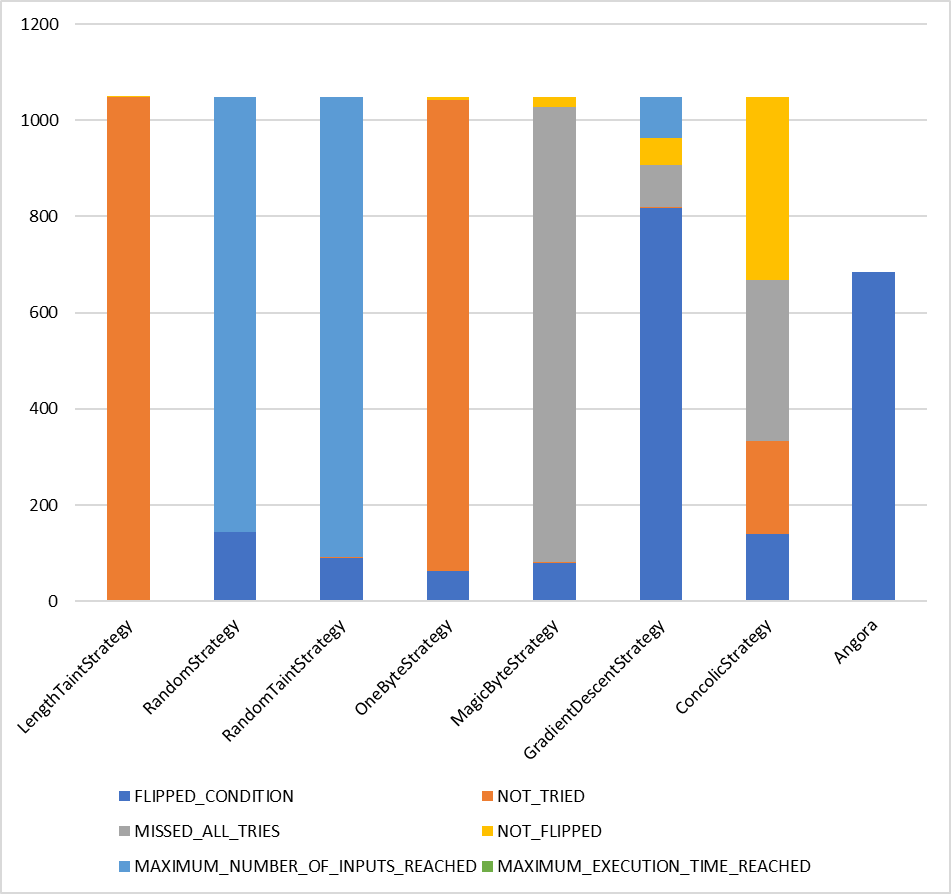
\includegraphics[width=.8\linewidth]{5_results/graphs/jhead-status.png}  
        \caption{Number of conditions flipped in the  \texttt{jhead} binary.}
        \label{fig:jheadStatus}
    \end{subfigure}
    \hfill
    \begin{subfigure}[b]{0.49\textwidth}
        \centering
        % include first image
        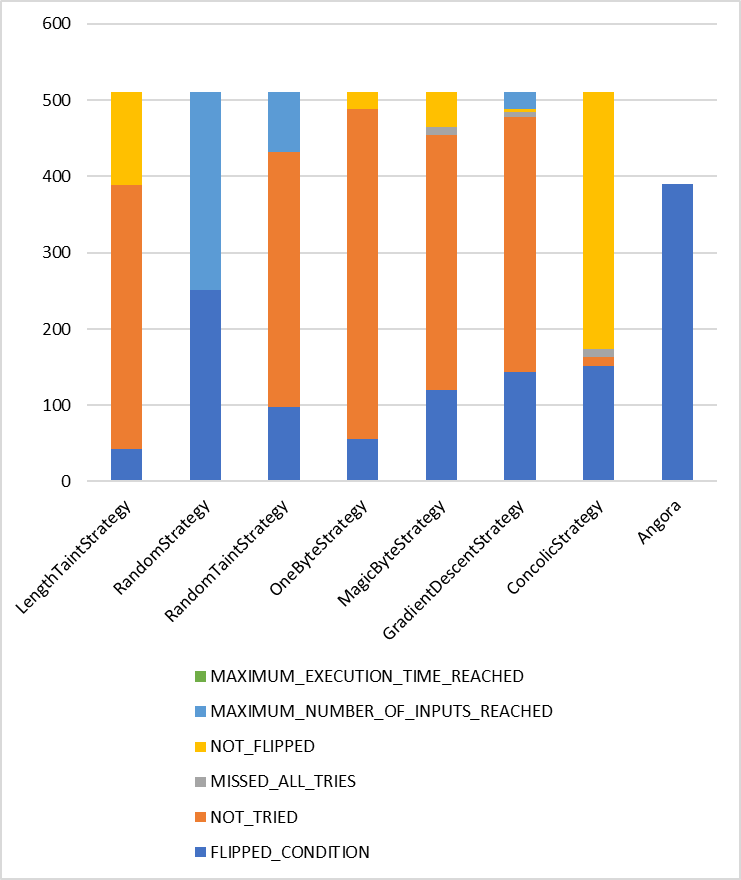
\includegraphics[width=.8\linewidth]{5_results/graphs/djpeg-status.png}  
        \caption{Number of conditions flipped in the  \texttt{djpeg} binary.}
        \label{fig:djpegStatus}
    \end{subfigure}
    \hfill
    \begin{subfigure}[b]{0.49\textwidth}
        \centering
        % include first image
        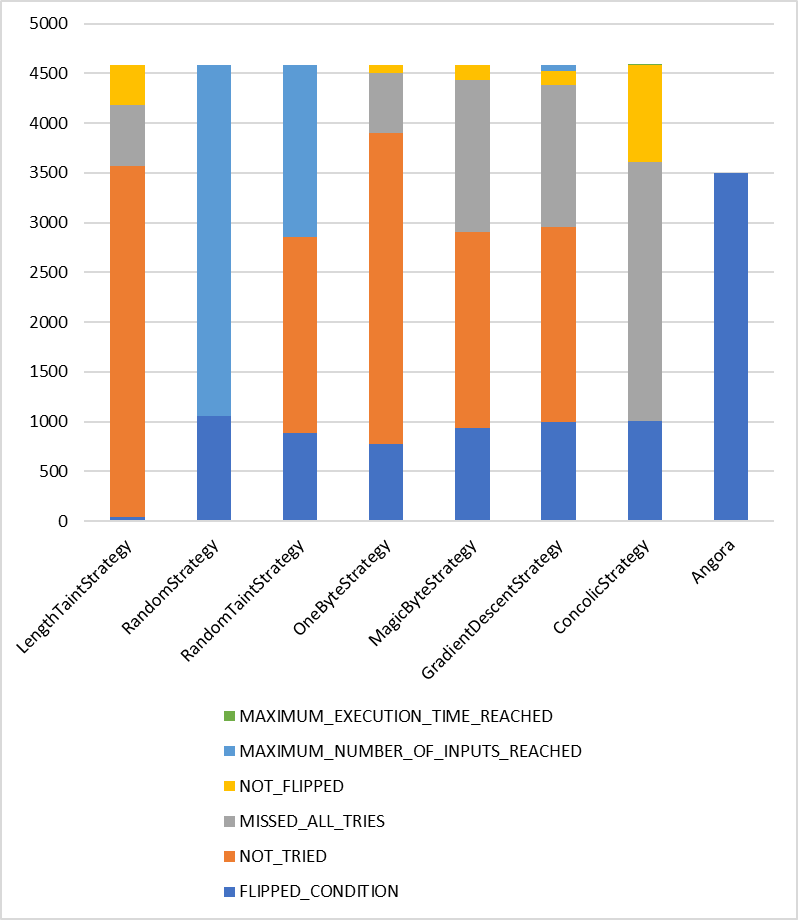
\includegraphics[width=.8\linewidth]{5_results/graphs/file-status.png}  
        \caption{Number of conditions flipped in the  \texttt{file} binary.}
        \label{fig:fileStatus}
    \end{subfigure}
    \hfill
    \begin{subfigure}[b]{0.49\textwidth}
        \centering
        % include first image
        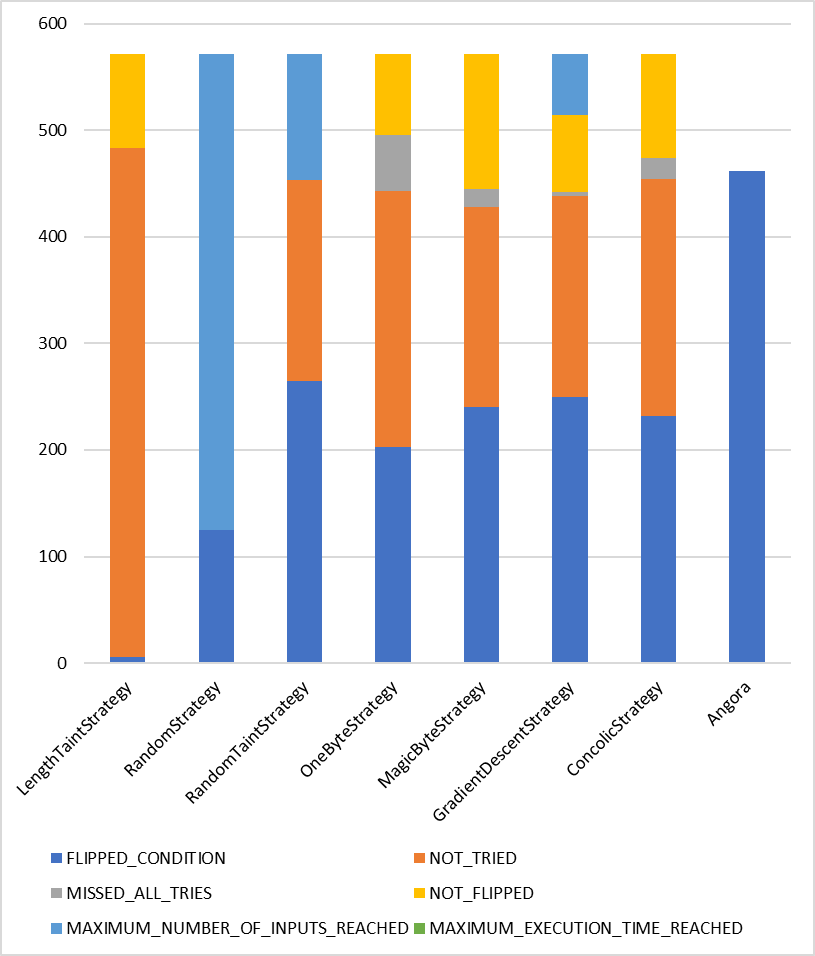
\includegraphics[width=.8\linewidth]{5_results/graphs/gif2png-status.png}  
        \caption{Number of conditions flipped in the  \texttt{gif2png} binary.}
        \label{fig:gif2pngStatus}
    \end{subfigure}
\caption{Number of conditions flipped per binary.}
\end{figure}

\begin{figure}[H]
    \centering
    \begin{subfigure}[b]{0.49\textwidth}
        \centering
        % include first image
        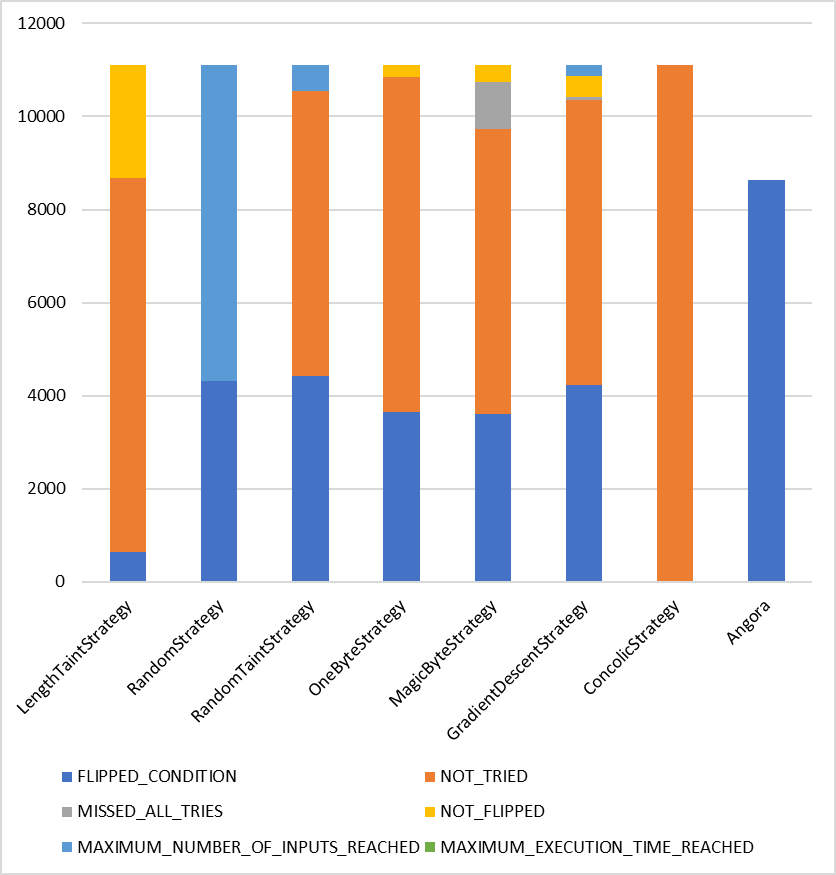
\includegraphics[width=.8\linewidth]{5_results/graphs/xmlwf-status.png}  
        \caption{Number of conditions flipped in the  \texttt{xmlwf} binary.}
        \label{fig:xmlwfStatus}
    \end{subfigure}
    \hfill
    \begin{subfigure}[b]{0.49\textwidth}
        \centering
        % include first image
        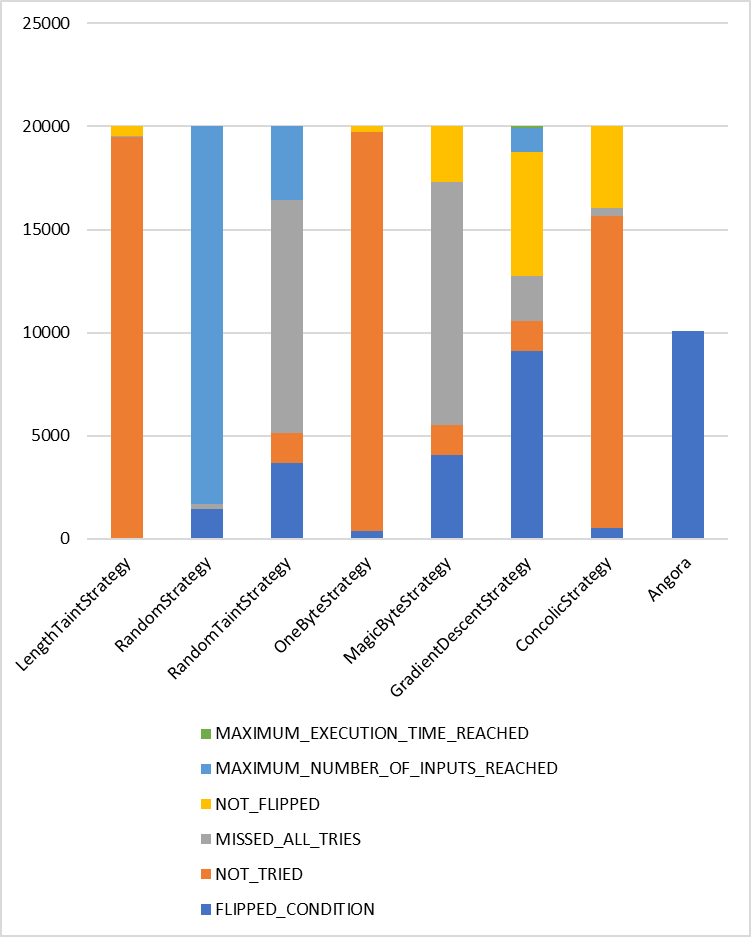
\includegraphics[width=.8\linewidth]{5_results/graphs/nm-status.png}  
        \caption{Number of conditions flipped in the \texttt{nm} binary.}
        \label{fig:nmStatus}
    \end{subfigure}
    \caption{Number of conditions flipped per binary.}
\end{figure}
When we compare the number of flips to the number of flips by Angora, we notice that only for the \texttt{jhead} program there are more flips found by our implemented strategies, than by Angora. This is mostly due to the flips found by the GradientDescent strategy, which outperforms all other strategies in this case as seen in Figure \ref{fig:djpegStatus}.

However, if we look at the \texttt{file} program, we see quite the opposite. We found only 30\% of all the flips found by Angora. And quite surprisingly the RandomStrategy, without any taint information, finds the most flips of all other strategies and the GradientDescent strategy finds nearly as many flips as the RandomTaintStrategy as seen in Figure \ref{fig:fileStatus}. 

This results seems to repeat itself in the \texttt{gif2png} program, where now the RandomTaintStrategy performs only better than the LengthTaintStrategy, but again there is little difference in total flips between the GradientDescentStrategy and the RandomTaintStrategy as seen in Figure \ref{fig:gif2pngStatus}.


In the \texttt{djpeg} program, again the RandomStrategy performs best, while now the Concolic and GradientDescent strategies compete for the second place as seen in Figure \ref{fig:djpegStatus}.

As seen in Figure \ref{fig:xmlwfStatus} \texttt{xmlwf} program, the RandomStrategy, RandomTaintStrategy and GradientDescent strategy perform about equally good, while the OneByte and MagicByte strategies are close for the second best strategy.

In the \texttt{nm} binary, as seen in Figure \ref{fig:nmStatus}, we see that the GradientDescent outperforms all other strategies, and we find a number of flips nearly equal to Angora.



\begin{figure}[H]
    \centering
    % include first image
    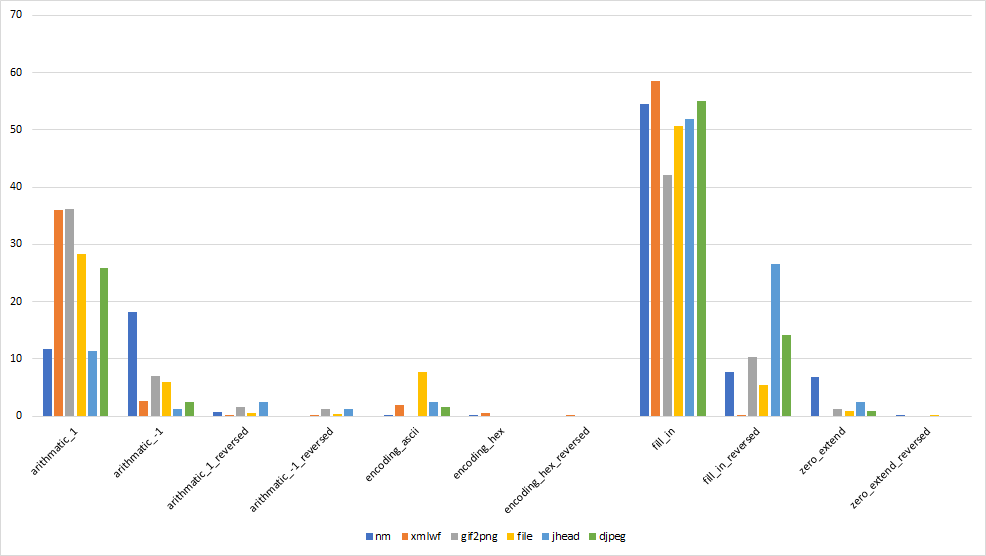
\includegraphics[width=.8\linewidth]{5_results/graphs/magic-byte-substrategy.png}  
    \caption{Number of flipped conditions using the MagicByte strategy per substrategy.}
    \label{fig:magicByteSubstrategies}
\end{figure}
We also made an overview of the substrategies used to flip a branch in the MagicByte strategy. We see clearly that filling in the magic bytes or using one-off values performs relatively well as substrategy. Also reversing a filled in value seems to work and converting the value to ASCII. We also see a difference between the programs which were checked. The \texttt{jhead} program seems to use more reversed statements, while the file program has more checks in ASCII values. The \texttt{nm} program has more flips by adding $-1$ to the value being compared.


\begin{figure}[H]
    \centering
    % include first image
    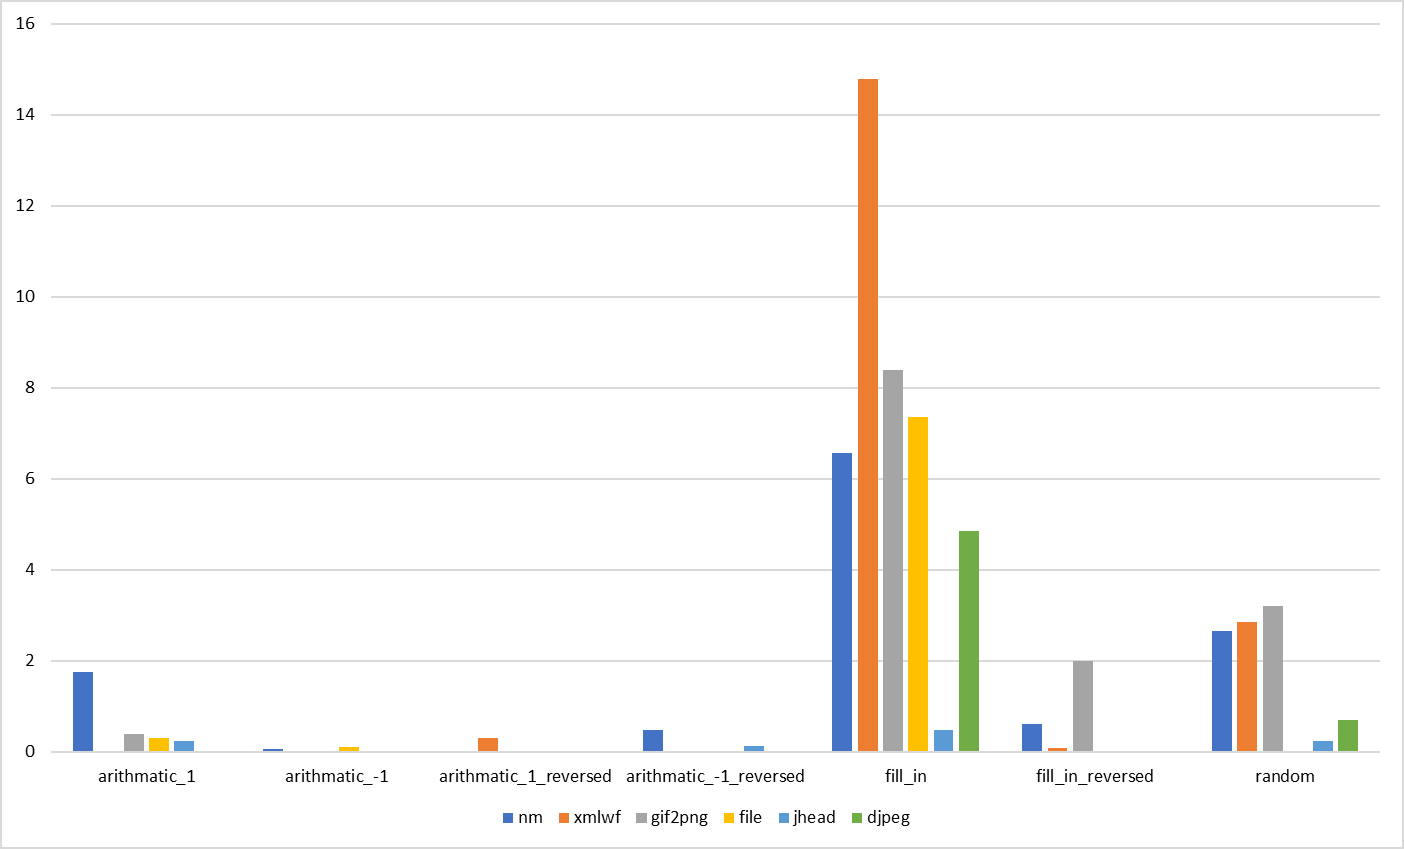
\includegraphics[width=.8\linewidth]{5_results/graphs/gradient-descent-substrategy.png}  
    \caption{Number of flipped conditions using the GradientDescent strategy per substrategy.}
    \label{fig:gradientDescentSubstrategies}
\end{figure}
We also made an overview of the substrategies used to flip a branch in the GradientDescent strategy. We see that it is most effective to use the value to be compared to in the \texttt{xmlwf} binary, however, most flips came from the initial value being compared.

From these graphs, we do not see a consistent result where one strategy outperform the another. We do see however, that the GradientDescent strategy works well in some cases like \texttt{jhead} and \texttt{nm} and that the RandomStrategy still finds a number of flips comparable to more sophisticated strategies.

From the comparison of the substrategies, we see that just filling in the bytes found in the comparison of a condition or doing this with one added or subtracted is a very effective way of flipping a condition, which supports the results from Redqueen \cite{aschermann2019redqueen}. 

From the comparison of the GradientDescent strategy, we see that combining this with the MagicByte strategy finds some new flips, so a combination of these strategies is a valid option as an improved GradientDescent strategy.


\section{Static Metrics}
In this section we will look at the results of the static metrics, namely the cyclomatic complexity, the Oviedo complexity, the chain size and the number of cases. An explanation of the metrics can be found in Section \ref{subsec:designStaticMetrics}. We assume that if we measure the same value from one of these metrics, the conditions have something in common. So we group all of these conditions together and we calculate the fraction of these which we flipped. For example, all conditions with an Oviedo complexity of 10 are grouped together and the fraction of flipped conditions is calculated. We do this for every metric.
We want to know if these metrics are correlated with the number of flips. To find such a relation, we use a correlation test. This can only be performed under the assumption that the values come from a normal distribution. 

We test if the correlation coefficient equals 0 as our null hypothesis with a confidence interval of 0.05. Our alternative hypothesis is that the correlation coefficient does not equal 0.

This test is done on the created pairs of conditions with the same value for the metric. For example, if there were only 2 possible values for the cyclomatic complexity, the sample size of the test equals 2. So even though we can have a lot of data which went into constructing the pairs, the number of unique values in the measurements influences the required correlation coefficient for a significant result.
We will give the correlation coefficient of all the metrics split by program, and a red background indicates a statistically significant result.
\todo{nrOfOffsets is dynamic, remove from table}


    \begin{table}[H]
    \centering
    \begin{tabular}{llllllll}
&  Ovie&Cycl&Offs&Cases&Chain&AbsD&RelD\\
GradientDescentStrategy&\cellcolor[HTML]{FFC7CE}{\color[HTML]{9C0006}0.0}&\cellcolor[HTML]{FFC7CE}{\color[HTML]{9C0006}0.0}&\cellcolor[HTML]{FFC7CE}{\color[HTML]{9C0006}0.0}&\cellcolor[HTML]{FFC7CE}{\color[HTML]{9C0006}0.01}&\cellcolor[HTML]{FFC7CE}{\color[HTML]{9C0006}0.02}&\cellcolor[HTML]{FFC7CE}{\color[HTML]{9C0006}0.05}&\cellcolor[HTML]{FFC7CE}{\color[HTML]{9C0006}0.0}\\
MagicByteStrategy&0.3&\cellcolor[HTML]{FFC7CE}{\color[HTML]{9C0006}0.01}&\cellcolor[HTML]{FFC7CE}{\color[HTML]{9C0006}0.0}&\cellcolor[HTML]{FFC7CE}{\color[HTML]{9C0006}0.0}&\cellcolor[HTML]{FFC7CE}{\color[HTML]{9C0006}0.0}&\cellcolor[HTML]{FFC7CE}{\color[HTML]{9C0006}0.0}&0.15\\
OneByteStrategy&0.34&\cellcolor[HTML]{FFC7CE}{\color[HTML]{9C0006}0.0}&\cellcolor[HTML]{FFC7CE}{\color[HTML]{9C0006}0.0}&\cellcolor[HTML]{FFC7CE}{\color[HTML]{9C0006}0.0}&\cellcolor[HTML]{FFC7CE}{\color[HTML]{9C0006}0.0}&\cellcolor[HTML]{FFC7CE}{\color[HTML]{9C0006}0.0}&\cellcolor[HTML]{FFC7CE}{\color[HTML]{9C0006}0.0}\\
LengthTaintStrategy&nan&nan&nan&nan&nan&nan&nan\\
ConcolicStrategy&\cellcolor[HTML]{FFC7CE}{\color[HTML]{9C0006}0.0}&\cellcolor[HTML]{FFC7CE}{\color[HTML]{9C0006}0.0}&0.11&\cellcolor[HTML]{FFC7CE}{\color[HTML]{9C0006}0.0}&\cellcolor[HTML]{FFC7CE}{\color[HTML]{9C0006}0.0}&0.41&0.12\\
RandomStrategy&0.22&0.2&0.12&\cellcolor[HTML]{FFC7CE}{\color[HTML]{9C0006}0.0}&\cellcolor[HTML]{FFC7CE}{\color[HTML]{9C0006}0.0}&\cellcolor[HTML]{FFC7CE}{\color[HTML]{9C0006}0.0}&0.05\\
RandomTaintStrategy&0.08&\cellcolor[HTML]{FFC7CE}{\color[HTML]{9C0006}0.0}&\cellcolor[HTML]{FFC7CE}{\color[HTML]{9C0006}0.0}&\cellcolor[HTML]{FFC7CE}{\color[HTML]{9C0006}0.0}&\cellcolor[HTML]{FFC7CE}{\color[HTML]{9C0006}0.0}&\cellcolor[HTML]{FFC7CE}{\color[HTML]{9C0006}0.0}&0.08\\

    \end{tabular}
    \caption{Significant difference of several metrics \texttt{jhead} binary}
    \label{tab:jheadWhitneyU}
    \end{table}
    
    
    
In Table \ref{tab:jheadCor}, the LengthTaintStrategy found no flips, hence the correlation coefficient was 0 everywhere.

\begin{table}[H]
    \centering
    \begin{tabular}{llllll}
\textbf{Correlation   coefficient} & nrOfOffsets & Cyclomatic & Oviedo   & Chain size & Cases    \\
GradientDescentStrategy            & 0,205318    & 0,011416   & 0,011457 & 0,21239     & -0,93573 \\
ConcolicStrategy                   & 0,631473    & -0,00485   & 0,000411 & 0,249513    & -0,74595 \\
MagicByteStrategy                  & 0,738903    & -0,03474   & -0,03581 & 0,099961    & -0,88598 \\
RandomStrategy                     & 0,745772    & 0,287292   & 0,26743  & 0,256173    & -0,88548 \\
RandomTaintStrategy                & -0,2137     & -0,02883   & -0,03515 & -0,03184    & -0,64501 \\
LengthTaintStrategy                & -0,44039    & 0,221465   & 0,253842 & 0,119641    & -0,5309  \\
OneByteStrategy                    & -0,33029    & -0,09256   & -0,10361 & -0,06478    & -0,56449 \\hline
Sample size                        & 4           & 10         & 11       & 32          & 3       
\end{tabular}
    \caption{Correlation coefficients of the \texttt{djpeg} binary}
    \label{tab:djpegCor}
\end{table}
\begin{table}[H]
    \centering
    \begin{tabular}{llllll}
\textbf{Correlation   coefficient} & nrOfOffsets & Cyclomatic & Oviedo   & Chain size                                            & Cases                                                   \\
GradientDescentStrategy            & -0,23907    & 0,113457   & 0,195891 & -0,24598                                               & \cellcolor[HTML]{FFC7CE}{\color[HTML]{9C0006} 0,731024} \\
ConcolicStrategy                   & -0,21984    & 0,069807   & 0,130543 & -0,2832                                                & 0,669845                                                \\
MagicByteStrategy                  & -0,21204    & 0,136656   & 0,200582 & -0,24097                                               & 0,66458                                                 \\
RandomStrategy                     & -0,27992    & 0,015236   & 0,119628 & \cellcolor[HTML]{FFC7CE}{\color[HTML]{9C0006} -0,3187} & 0,682533                                                \\
RandomTaintStrategy                & -0,18134    & 0,07412    & 0,173287 & -0,23057                                               & 0,680243                                                \\
LengthTaintStrategy                & -0,11651    & 0,299711   & 0,097546 & 0,14474                                                & -0,59245                                                \\
OneByteStrategy                    & -0,1145     & 0,016899   & 0,055826 & -0,21049                                               & 0,664689                                                \\hline
Sample size                        & 23          & 32         & 46       & 47                                                     & 8                                                      
\end{tabular}
    \caption{Correlation coefficients of the \texttt{file} binary}
    \label{tab:fileCor}
\end{table}
\begin{table}[H]
    \centering
   \begin{tabular}{llllll}
\textbf{Correlation   coefficient} & nrOfOffsets & Cyclomatic                                              & Oviedo                                                  & Chain size & Cases \\
GradientDescentStrategy            & -0,48226    & \cellcolor[HTML]{FFC7CE}{\color[HTML]{9C0006} 0,747139} & \cellcolor[HTML]{FFC7CE}{\color[HTML]{9C0006} 0,808394} & -0,06959    &       \\
ConcolicStrategy                   & -0,4523     & 0,573681                                                & 0,605348                                                & -0,06253    &       \\
MagicByteStrategy                  & -0,45436    & \cellcolor[HTML]{FFC7CE}{\color[HTML]{9C0006} 0,775257} & \cellcolor[HTML]{FFC7CE}{\color[HTML]{9C0006} 0,799827} & -0,25979    &       \\
RandomStrategy                     & 0,095591    & 0,563317                                                & 0,550047                                                & -0,26082    &       \\
RandomTaintStrategy                & -0,10081    & 0,597975                                                & 0,558925                                                & 0,270854    &       \\
LengthTaintStrategy                & -0,41188    & 0,589697                                                & 0,49245                                                 & -0,20071    &       \\
OneByteStrategy                    & 0,104705    & 0,631743                                                & 0,550275                                                & 0,029647    &       \\hline
Sample size                        & 7           & 8                                                       & 8                                                       & 11          & 2    
\end{tabular}
    \caption{Correlation coefficients of the \texttt{gif2png} binary}
    \label{tab:gif2pngCor}
\end{table}
In Table \ref{tab:gif2pngCor} there were only 2 possible values for the number of cases, hence the correlation coefficient could not be calculated.

\begin{table}[H]
    \centering
    \begin{tabular}{llllll}
\textbf{Correlation   coefficient} & nrOfOffsets                                             & Cyclomatic                                             & Oviedo                                                  & Chain size & Cases    \\
GradientDescentStrategy            & \cellcolor[HTML]{FFC7CE}{\color[HTML]{9C0006} 0,55746}  & -0,19821                                               & -0,22831                                                & 0,030608    & 0,402348 \\
ConcolicStrategy                   &                                                         &                                                        &                                                         &             &          \\
MagicByteStrategy                  & \cellcolor[HTML]{FFC7CE}{\color[HTML]{9C0006} -0,43595} & -0,17436                                               & -0,2191                                                 & -0,01083    & 0,433612 \\
RandomStrategy                     & \cellcolor[HTML]{FFC7CE}{\color[HTML]{9C0006} 0,497585} & 0,162392                                               & 0,174867                                                & 0,08793     & 0,391188 \\
RandomTaintStrategy                & \cellcolor[HTML]{FFC7CE}{\color[HTML]{9C0006} -0,5751}  & -0,16767                                               & -0,19832                                                & 0,069683    & 0,386711 \\
LengthTaintStrategy                & -0,19668                                                & \cellcolor[HTML]{FFC7CE}{\color[HTML]{9C0006} 0,45029} & \cellcolor[HTML]{FFC7CE}{\color[HTML]{9C0006} 0,461258} & 0,003246    & -0,36074 \\
OneByteStrategy                    & -0,19313                                                & -0,17576                                               & -0,21887                                                & 0,026968    & 0,397983 \\hline
Sample size                        & 38                                                      & 36                                                     & 53                                                      & 53          & 18      
\end{tabular}
    \caption{Correlation coefficients of the \texttt{xmlwf} binary}
    \label{tab:xmlwfCor}
\end{table}
\begin{table}[H]
    \centering
    \begin{tabular}{llllll}
\textbf{Correlation   coefficient} & nrOfOffsets                                             & Cyclomatic & Oviedo   & Chain size                                             & Cases    \\
GradientDescentStrategy            & -0,00653                                                & 0,159567   & 0,195467 & \cellcolor[HTML]{FFC7CE}{\color[HTML]{9C0006} -0,43679} & -0,60323 \\
ConcolicStrategy                   & 0,214441                                                & -0,10202   & 0,02986  & -0,01512                                                & -0,28962 \\
MagicByteStrategy                  & \cellcolor[HTML]{FFC7CE}{\color[HTML]{9C0006} -0,43907} & 0,228513   & 0,189986 & 0,195629                                                & -0,45239 \\
RandomStrategy                     & 0,158416                                                & -0,07771   & 0,009494 & \cellcolor[HTML]{FFC7CE}{\color[HTML]{9C0006} -0,3671}  & -0,11419 \\
RandomTaintStrategy                & \cellcolor[HTML]{FFC7CE}{\color[HTML]{9C0006} -0,37221} & 0,265475   & 0,178601 & -0,3011                                                 & -0,44465 \\
LengthTaintStrategy                & -0,22297                                                & 0,122727   & 0,052122 & -0,17033                                                & -0,38742 \\
OneByteStrategy                    & -0,21442                                                & 0,212724   & 0,217546 & -0,16366                                                & -0,32016 \\hline
Sample size                        & 51                                                      & 40         & 65       & 38                                                      & 6       
\end{tabular}
    \caption{Correlation coefficients of the \texttt{nm} binary}
    \label{tab:nmCor}
\end{table}

From these results, we see that no metric gave a consistent correlation with the number of flips in any binary with any strategy. The chain size gave 7 statistically significant results out of the 42 tests, however 3 of those occurred in the \texttt{xmlwf} binary, so we do not consider this enough to conclude something from this metric.
Unfortunately, it looks as if the chosen static metrics do not give enough insight in the conditions to relate directly with the performance of a strategy. In the next section we will try to find a relation with the dynamic metrics.

\section{Dynamic metrics}
In this section we will look at the results of each strategy per binary in terms of depth, number of tainted bytes present in the condition, and time spend calculating the inputs. 
As we have seen in the overall results, often the RandomStrategy outperforms more sophisticated strategies. We hope to find a reason why this is by looking at these statistics more closely. 
In order to say something about the effectiveness of a strategy, we look at the time spend on a strategy. 

\subsection{Depth}
In this section we will look at the absolute depth of the conditions flipped per strategy and the relative depth of the conditions flipped per strategy.
\paragraph{Absolute depth}
We will first look at the absolute depth. We look the longest trace as 100\% of the length, and placed the other conditions in ranges of 10\% based on this total.
The totals on which the percentages were calculated can be found in Appendix \ref{appendix:depth}. Since we exclude conditions which we have already seen, we notice that the distribution of unique conditions per bucket is not uniform. In the \texttt{nm} binary, nearly all unique conditions which are seen are present in the first bucket, while the last bucket only has 12 unique conditions, while the \texttt{djpeg} binary has a peak of unique conditions at the 50-70\% bucket while in the 10-20\% bucket there is not a single unique condition.
\begin{figure}[H]
    \centering
    % include first image
    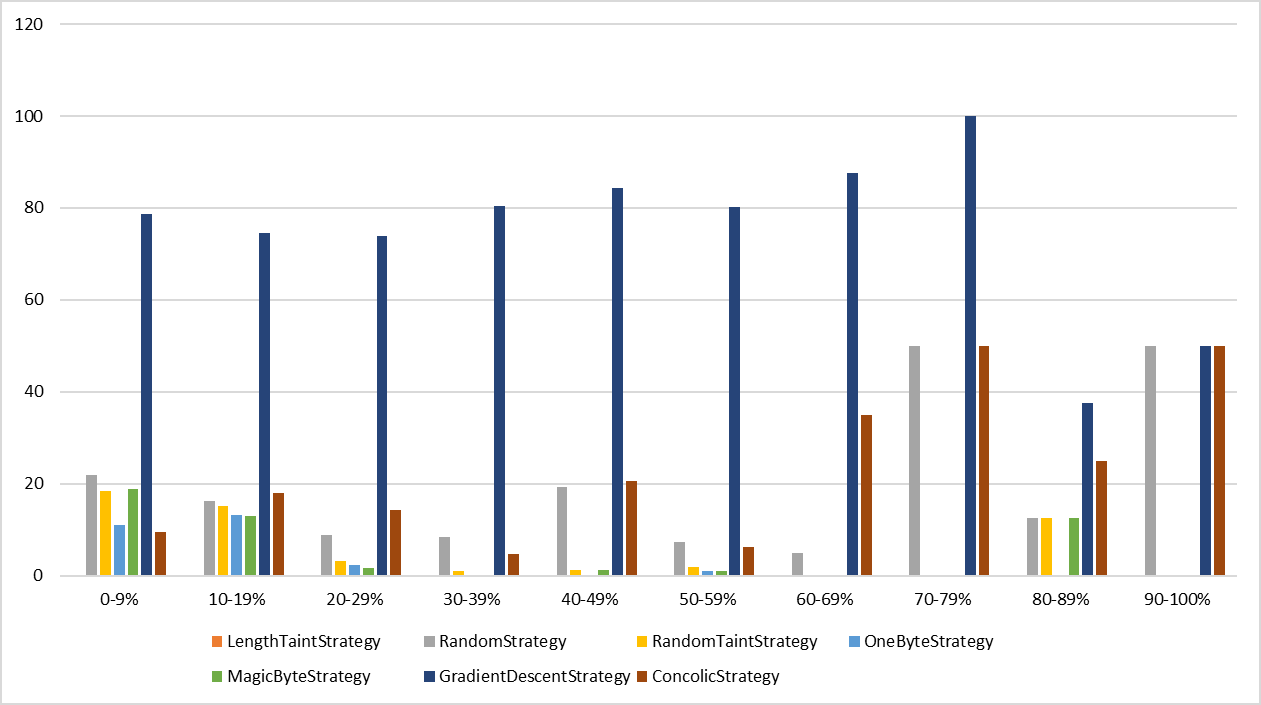
\includegraphics[width=.8\linewidth]{5_results/graphs/jhead-depth.png}  
    \caption{Percentage of flips per depth in the \texttt{jhead} binary.}
    \label{fig:jheadDepth}
\end{figure}
We see  in Figure \ref{fig:jheadDepth} that the GradientDescent strategy outperforms the other strategies at nearly every depth. We also see that the RandomStrategy seems to be on par, or sometimes better than the ConcolicStrategy per depth.
\begin{figure}[H]
    \centering
    % include first image
    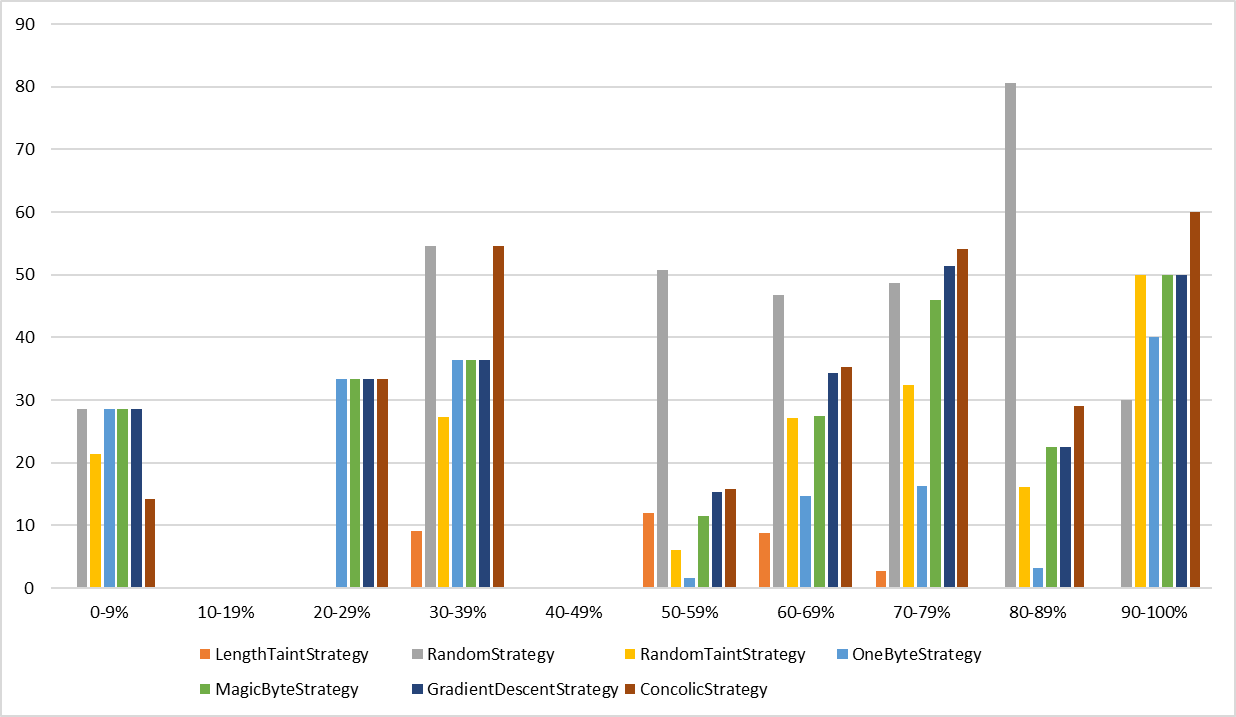
\includegraphics[width=.8\linewidth]{5_results/graphs/djpeg-depth.png}  
    \caption{Percentage of flips per depth in the \texttt{djpeg} binary.}
    \label{fig:djpegDepth}
\end{figure}
In Figure \ref{fig:djpegDepth} we see that the ConcolicStrategy seems to perform pretty good deeper in the program. An unexpected result is that the RandomStrategy seems to be out performing the other strategies in the 80-90\% bucket.
\begin{figure}[H]
    \centering
    % include first image
    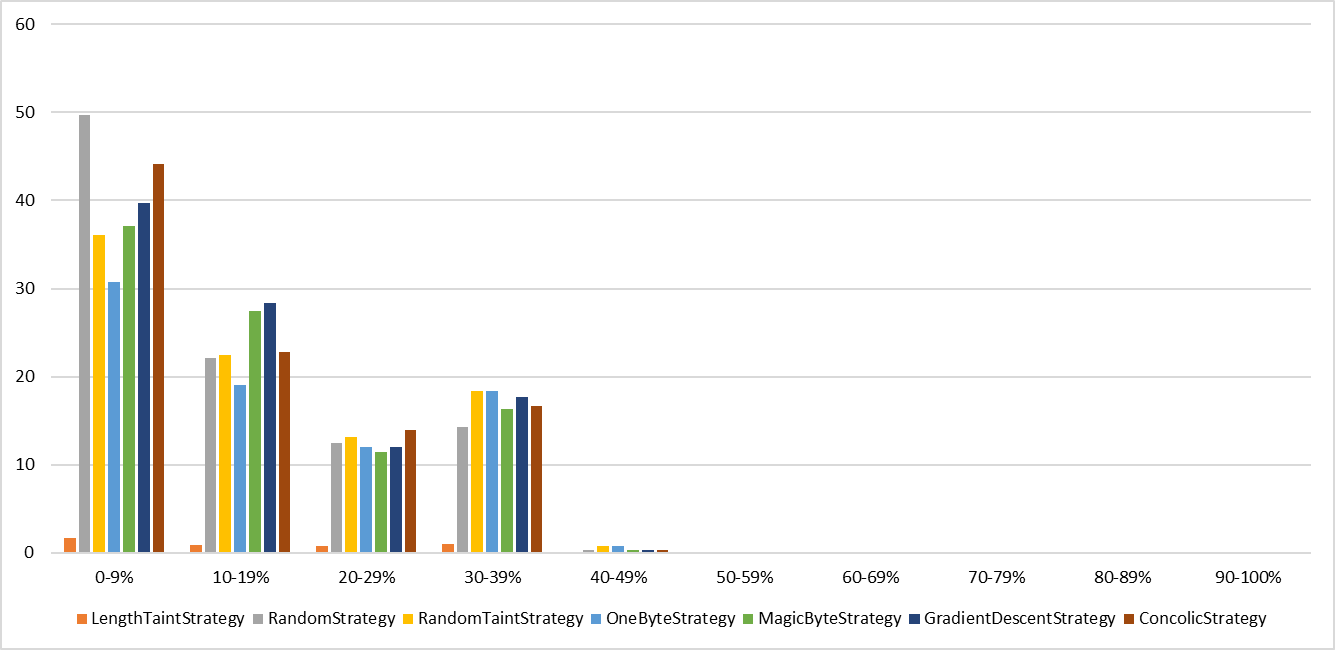
\includegraphics[width=.8\linewidth]{5_results/graphs/file-depth.png}  
    \caption{Percentage of flips per depth in the \texttt{file} binary.}
    \label{fig:fileDepth}
\end{figure}
In the \texttt{file} binary, we see that the metric we used for depth might be sensitive to outliers in Figure \ref{fig:fileDepth}. We will discuss this metric in depth in Chapter \ref{chap:discussion}, but it seems that if there has been 1 long trace, most shorter traces fall in the earlier buckets. In these buckets, we see in the first bucket a large impact of the RandomStrategy, which decreases when the depth decreases, but in the 30-40\% bucket, the number of flips seems to increase followed by a quick decrease in the number of flipped conditions. We checked if this could have something to do with losing taint information, but this was not the case.
\begin{figure}[H]
    \centering
    % include first image
    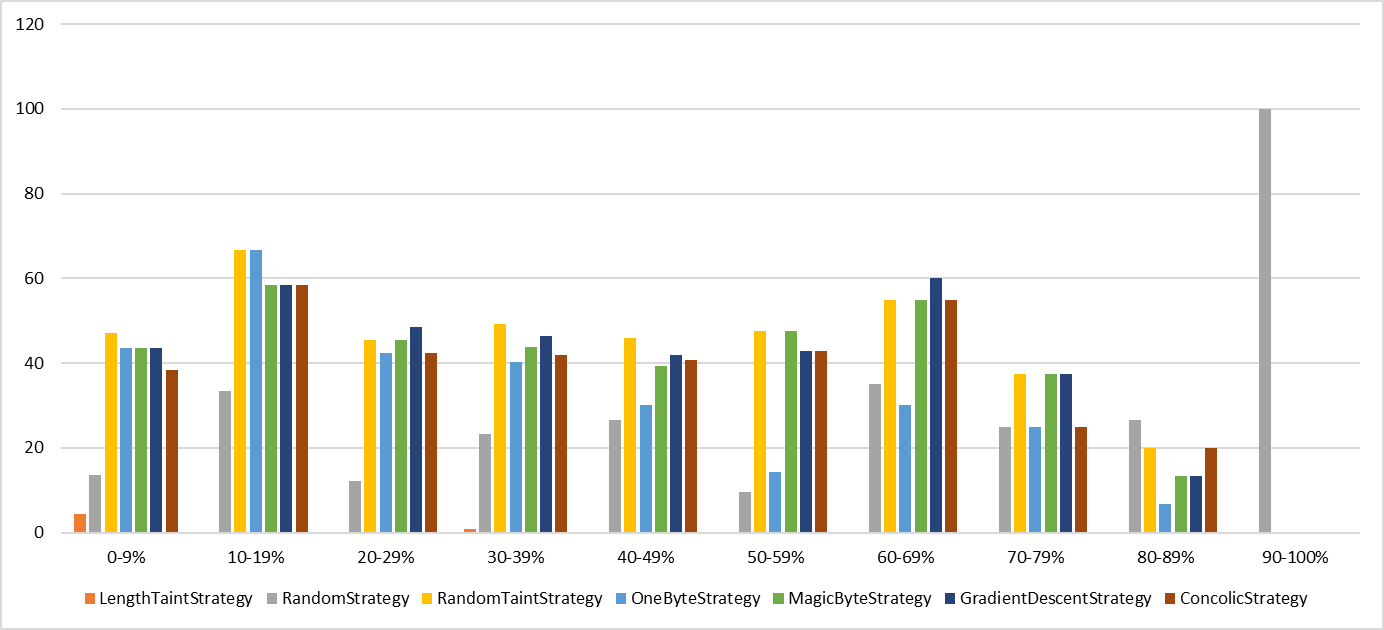
\includegraphics[width=.8\linewidth]{5_results/graphs/gif2png-depth.png}  
    \caption{Percentage of flips per depth in the \texttt{gif2png} binary.}
    \label{fig:gif2pngDepth}
\end{figure}
When we look at the depth of the results of the percentage of flips of the \texttt{gif2png} binary in Figure \ref{fig:gif2pngDepth}, we notice that most strategies perform equally well per depth, but in the final bucket only the RandomStrategy manages to flip conditions. There were only 4 conditions flipped in this last bucket, which were all flipped by this strategy, so this might skew with the results, again we will discuss this metric in Chapter \ref{chap:discussion}.
\begin{figure}[H]
    \centering
    % include first image
    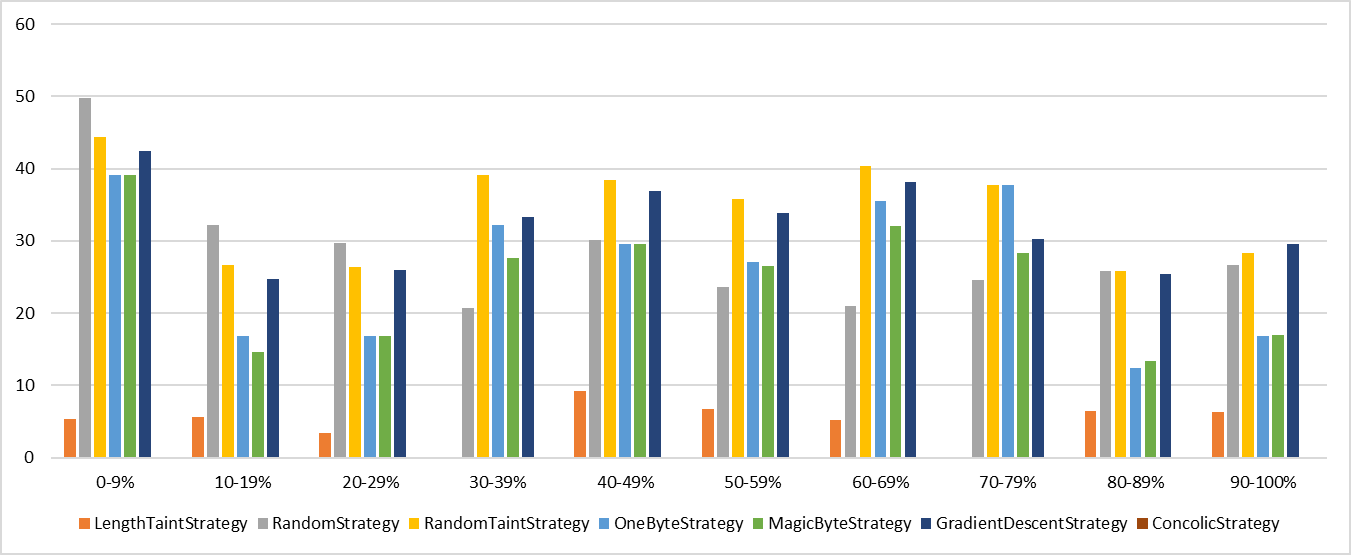
\includegraphics[width=.8\linewidth]{5_results/graphs/xmlwf-depth.png}  
    \caption{Percentage of flips per depth in the \texttt{xmlwf} binary.}
    \label{fig:xmlwfDepth}
\end{figure}
The \texttt{xmlwf} binary has a pretty even distribution of the number of flips. This could be attributed to the structure of the program, which checks if something is a valid XML file. If this is done recursively, the same strategies could mutate the elements of the xml in somewhat the same way. We see that the RandomTaint strategy performs better or better than the GradientDescent strategy.
\begin{figure}[H]
    \centering
    % include first image
    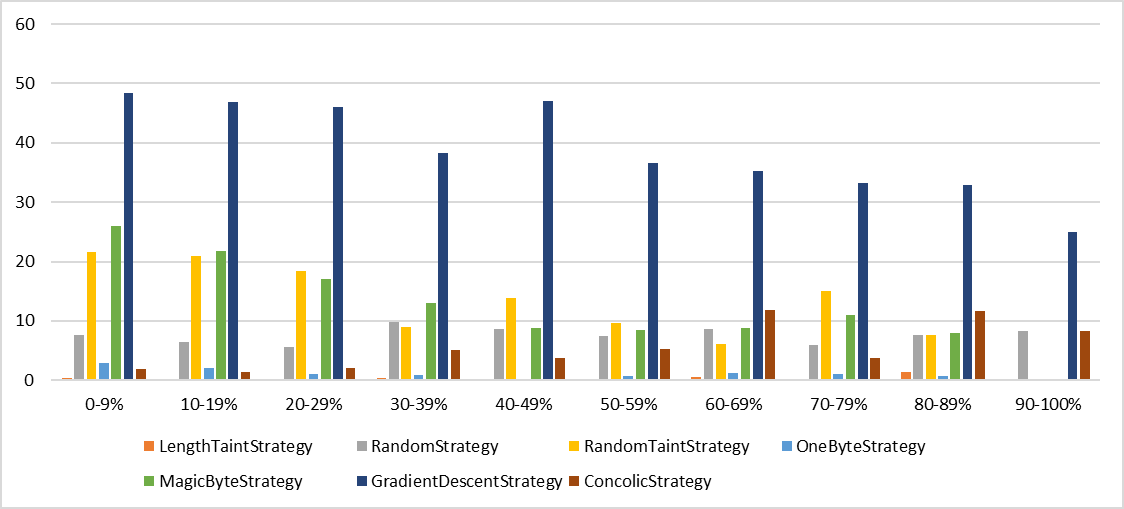
\includegraphics[width=.8\linewidth]{5_results/graphs/nm-depth.png}  
    \caption{Percentage of flips per depth in the \texttt{nm} binary.}
    \label{fig:nmDepth}
\end{figure}
In the \texttt{nm} binary, we see that the GradientDescent strategy outperforms nearly all other strategies with nearly twice as many flipped conditions than all others. We also see the ConcolicStrategy increasing if we are deeper in the program.

We again see that fr the \texttt{nm} and \texttt{jhead} programs the GradientDescent strategy works best, but for other programs this differs. Also the ConcolicStrategy works better deeper in the program, which is an expected result. However, for some programs like \texttt{djpeg} the RandomStrategy performs better than expected on multiple depths. Further research is required to see why this happens for this program.

\paragraph{Relative depth}
We also looked at the depth of a condition in a trace, and we placed all these conditions in buckets of 10\% based on their position in the corresponding trace.
\begin{figure}[H]
    \centering
    % include first image
    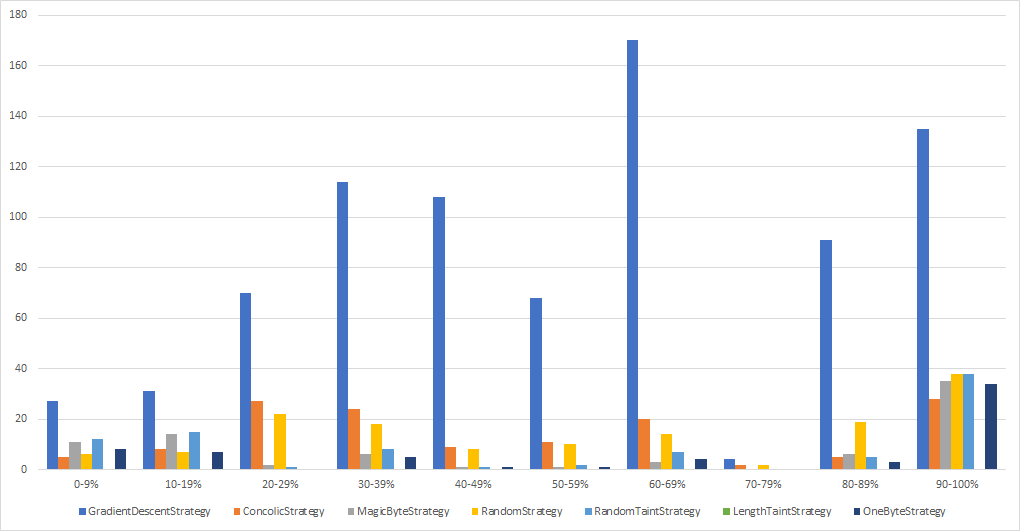
\includegraphics[width=.8\linewidth]{5_results/graphs/jhead-depth-relative.png}  
    \caption{Percentage of flips per relative depth in the \texttt{jhead} binary.}
    \label{fig:jheadDepthRelative}
\end{figure}
When we look at the performance of the GradientDescentStrategy in Figure \ref{fig:jheadDepthRelative}, we see that it outperforms most other strategies. It is interesting to note that the number of flips is not uniform in the trace, at the \texttt{70-79\%} bucket, there are hardly any flips found.

\begin{figure}[H]
    \centering
    % include first image
    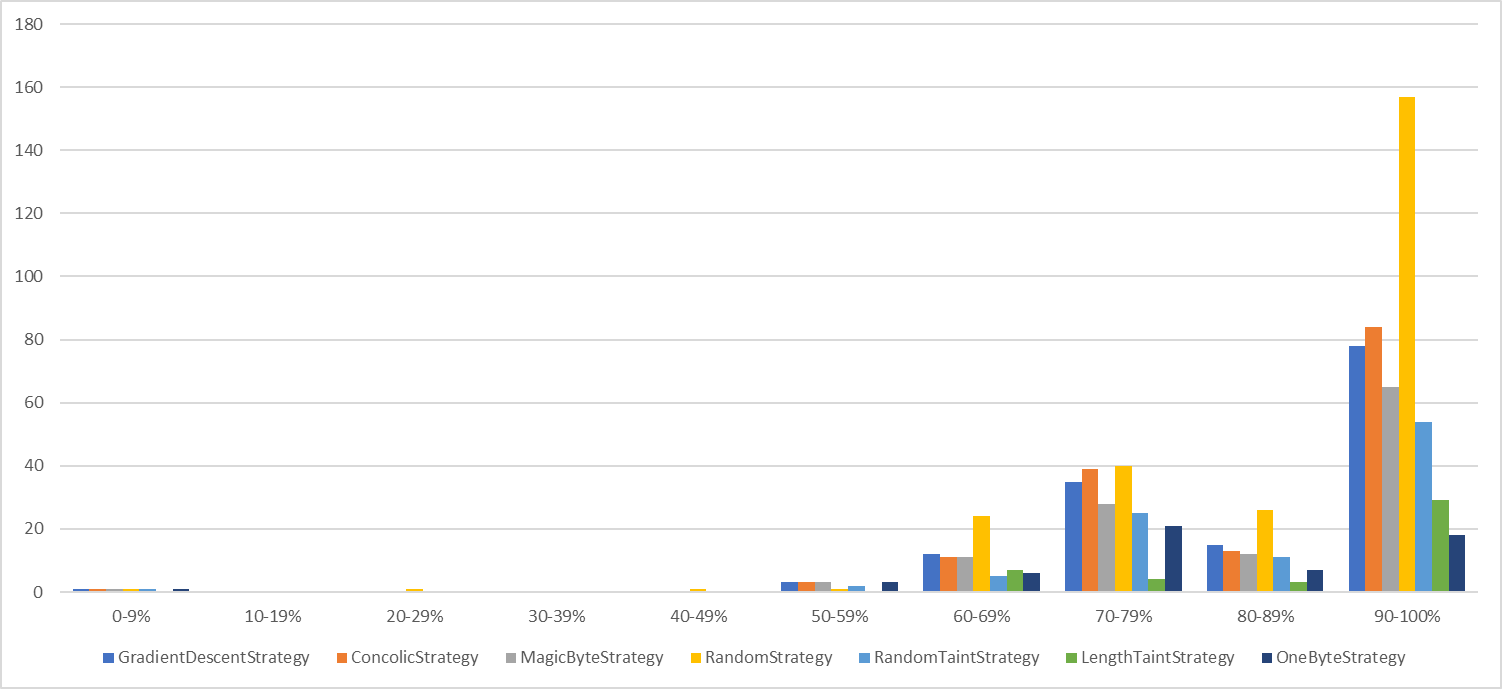
\includegraphics[width=.8\linewidth]{5_results/graphs/djpeg-depth-relative.png}  
    \caption{Percentage of flips per relative depth in the \texttt{djpeg} binary.}
    \label{fig:djpegDepthRelative}
\end{figure}
In Figure \ref{fig:jheadDepthRelative}, it appears as if the entire first \texttt{50\%} of the program has very little flips, and only at the end of the program do there appear to be flips, where the RandomStrategy outperforms the other strategies.


\begin{figure}[H]
    \centering
    % include first image
    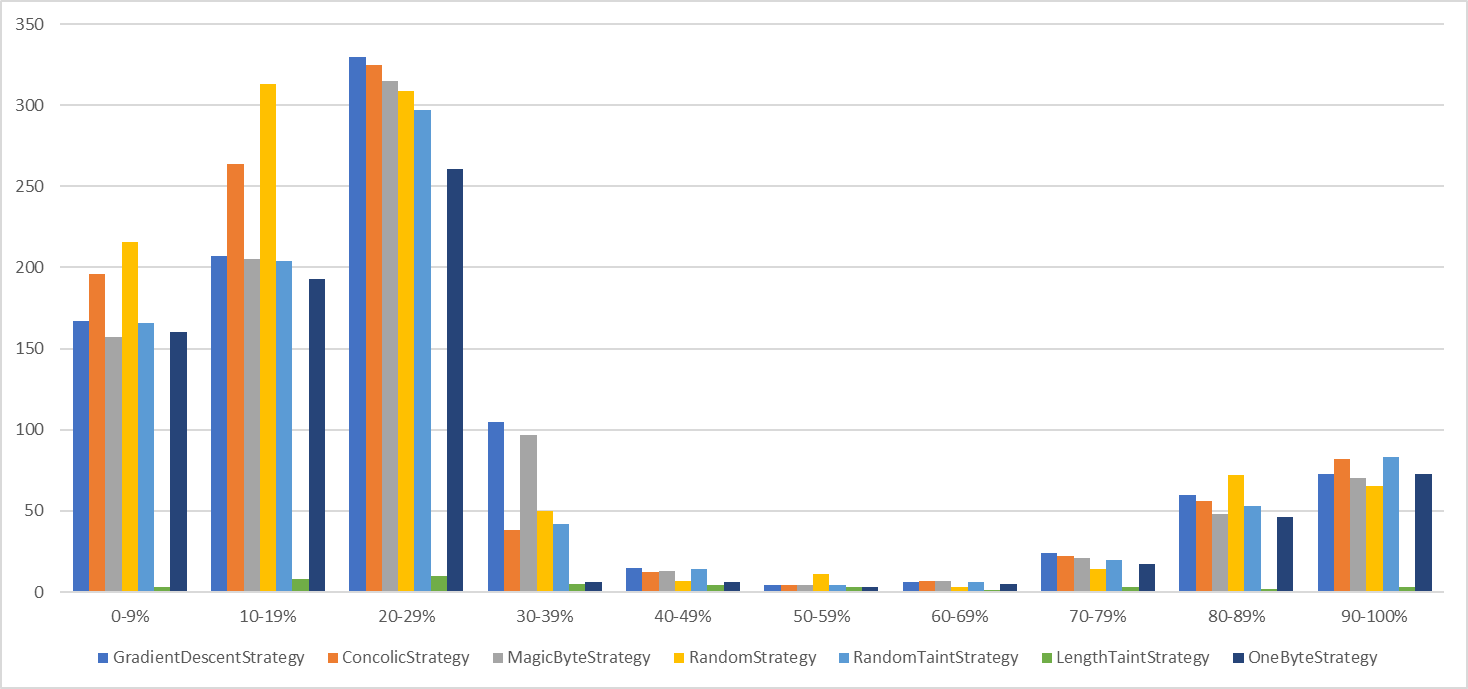
\includegraphics[width=.8\linewidth]{5_results/graphs/file-depth-relative.png}  
    \caption{Percentage of flips per relative depth in the \texttt{file} binary.}
    \label{fig:fileDepthRelative}
\end{figure}
It is interesting to see that with the relative depth we get a better sense of where in the traces the flips occur. In Figure \ref{fig:fileDepthRelative}, we see that in the first \texttt{30\%} buckets most flips of the program occur, then a decrease in the number of flips and then towards the end again more flips.

\begin{figure}[H]
    \centering
    % include first image
    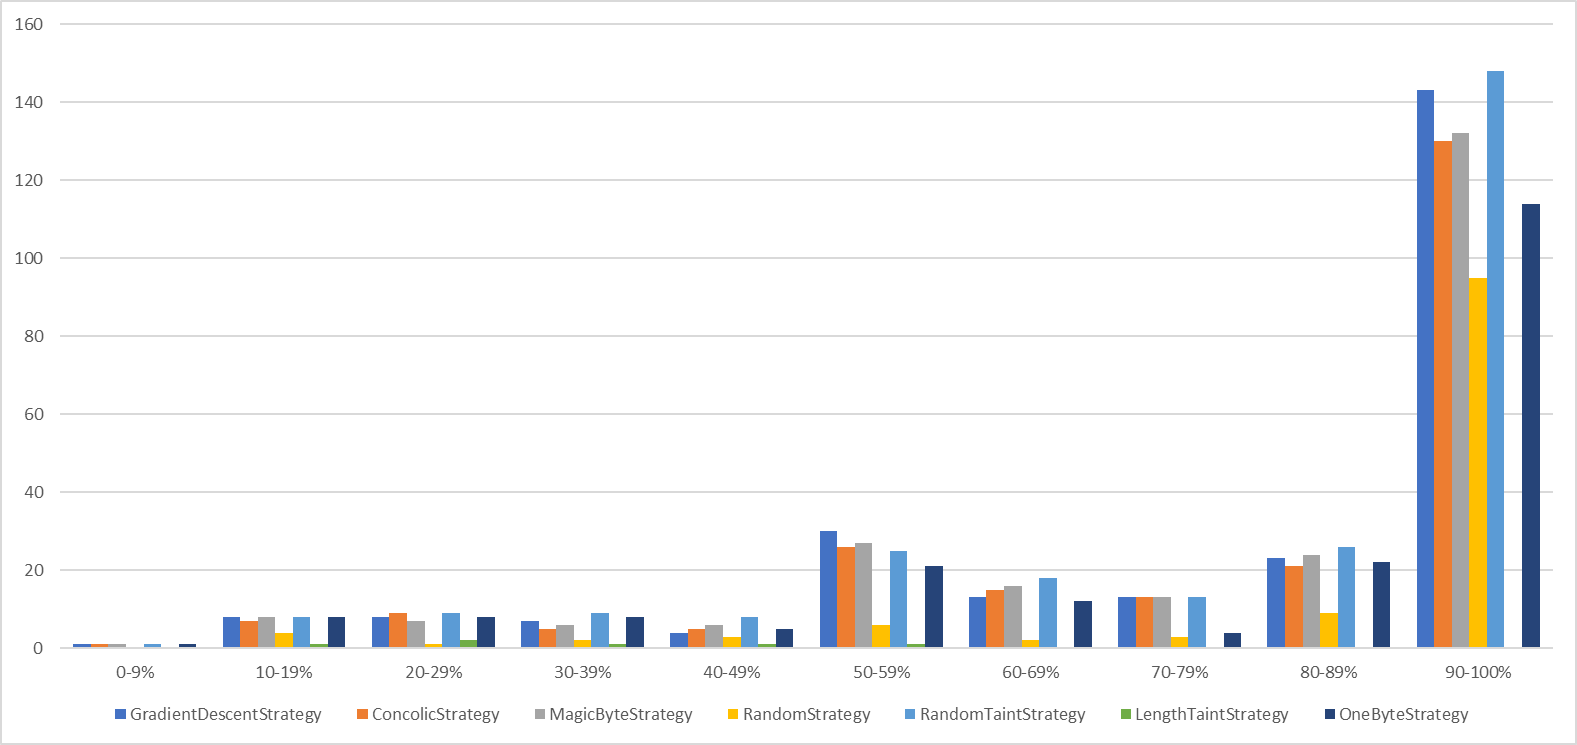
\includegraphics[width=.8\linewidth]{5_results/graphs/gif2png-depth-relative.png}  
    \caption{Percentage of flips per relative depth in the \texttt{gif2png} binary.}
    \label{fig:gif2pngDepthRelative}
\end{figure}
In the relative depth of the \texttt{gif2png} binary in Figure \ref{fig:gif2pngDepthRelative}, we notice that most flips occur in the last part of the traces, while there are hardly any flips in the first part of the program.

\todo{xmlwf is missing}

\begin{figure}[H]
    \centering
    % include first image
    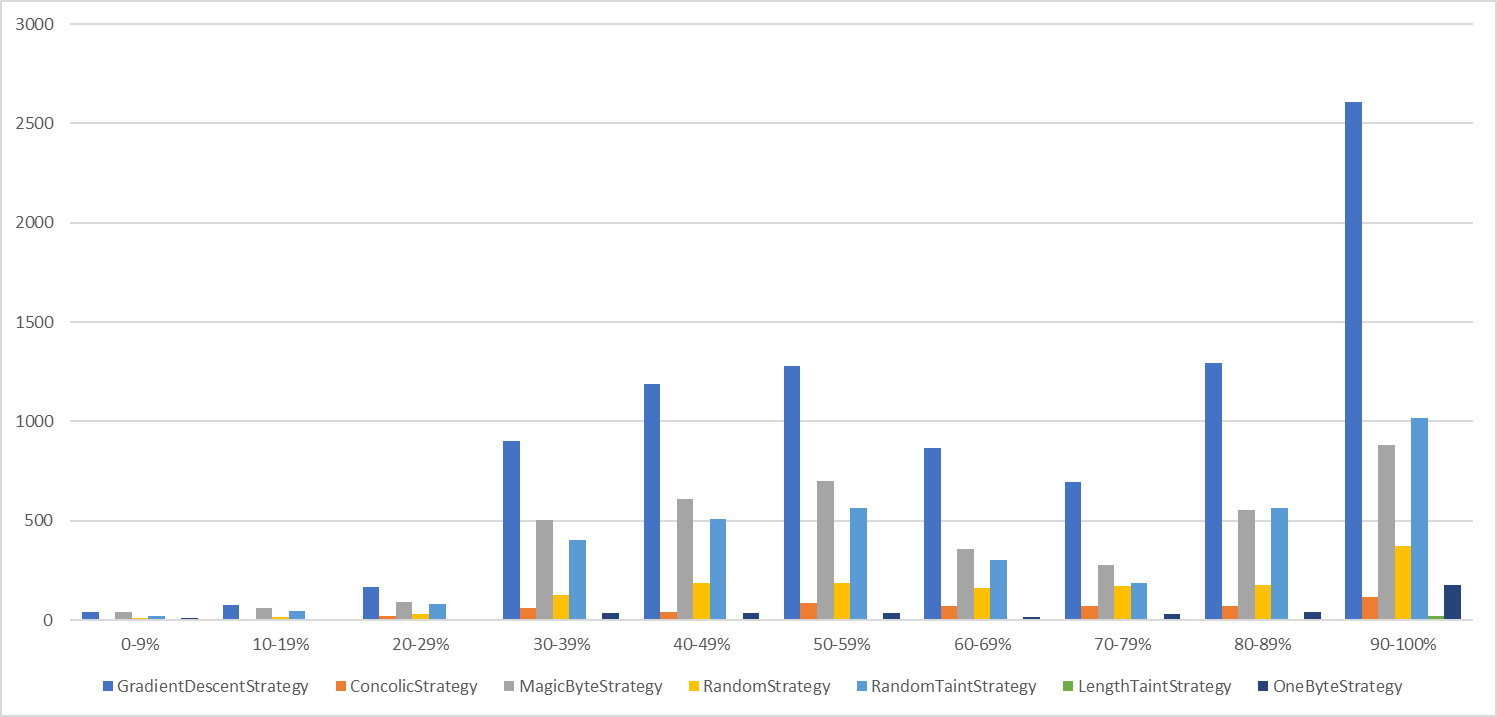
\includegraphics[width=.8\linewidth]{5_results/graphs/nm-depth-relative.png}  
    \caption{Percentage of flips per relative depth in the \texttt{nm} binary.}
    \label{fig:nmDepthRelative}
\end{figure}
In Figure \ref{fig:nmDepthRelative}, we see that the GradientDescentStrategy outperforms most other strategies, especially in the last bucket of the traces.

\subsection{Offsets}
In this subsection we will look at the results of the comparison of the strategies in binaries when looking at the number of offsets present in a condition. We take the total number of conditions per offset as 100\% and look at the relative performance of each strategy. The totals on which the percentages were calculated can be found in Appendix \ref{appendix:offsets}.
\begin{figure}[H]
    \centering
    % include first image
    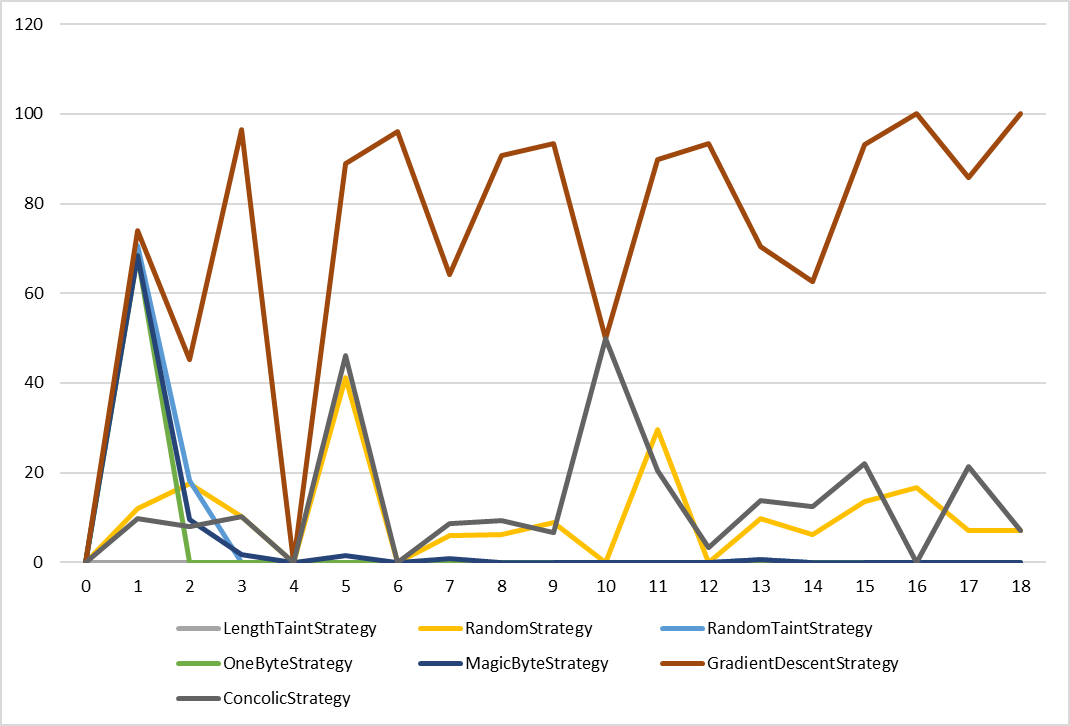
\includegraphics[width=.8\linewidth]{5_results/graphs/jhead-offsets.png}  
    \caption{Percentage of conditions flipped per number of offsets present from the input in the \texttt{jhead} binary.}
    \label{fig:jheadOffsets}
\end{figure}
We see some interesting behaviour of the GradientDescent strategy in Figure \ref{fig:jheadOffsets}, which outperforms all other strategies for every number of offsets present. We also see that the Concolic and Random stragies still find flips when more offsets are present in the condition. Most strategies find flips when only 1 offset from the input is present.
\begin{figure}[H]
    \centering
    % include first image
    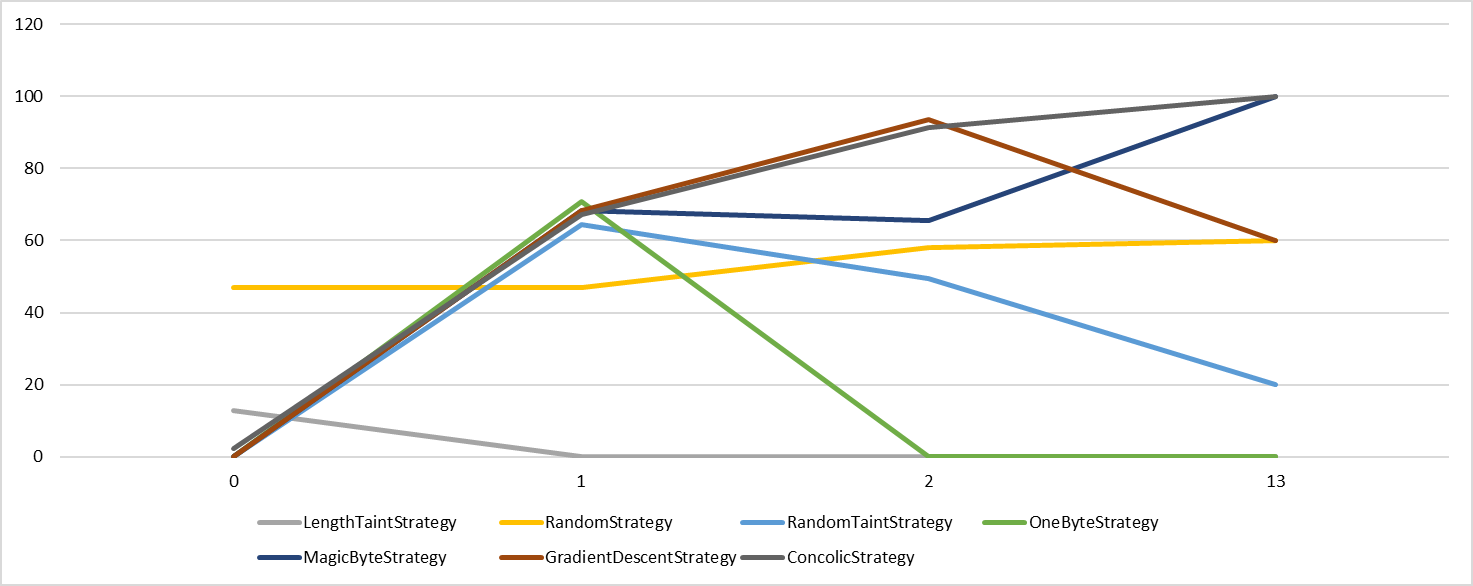
\includegraphics[width=.8\linewidth]{5_results/graphs/djpeg-offsets.png}  
    \caption{Percentage of conditions flipped per number of offsets present from the input in the \texttt{djpeg} binary.}
    \label{fig:djpegOffsets}
\end{figure}
Again we see that most strategies find flips with 1 offset in Figure \ref{fig:djpegOffsets}. What is interesting, is that the RandomStrategy seems to find way more flips when no offsets are present than the other strategies. After this, it is outperformed by other strategies. However, this might indicate that some taint has been lost during the execution of the \texttt{djpeg} runs, since here the input influences the conditions, while no offsets from the input were found.
\begin{figure}[H]
    \centering
    % include first image
    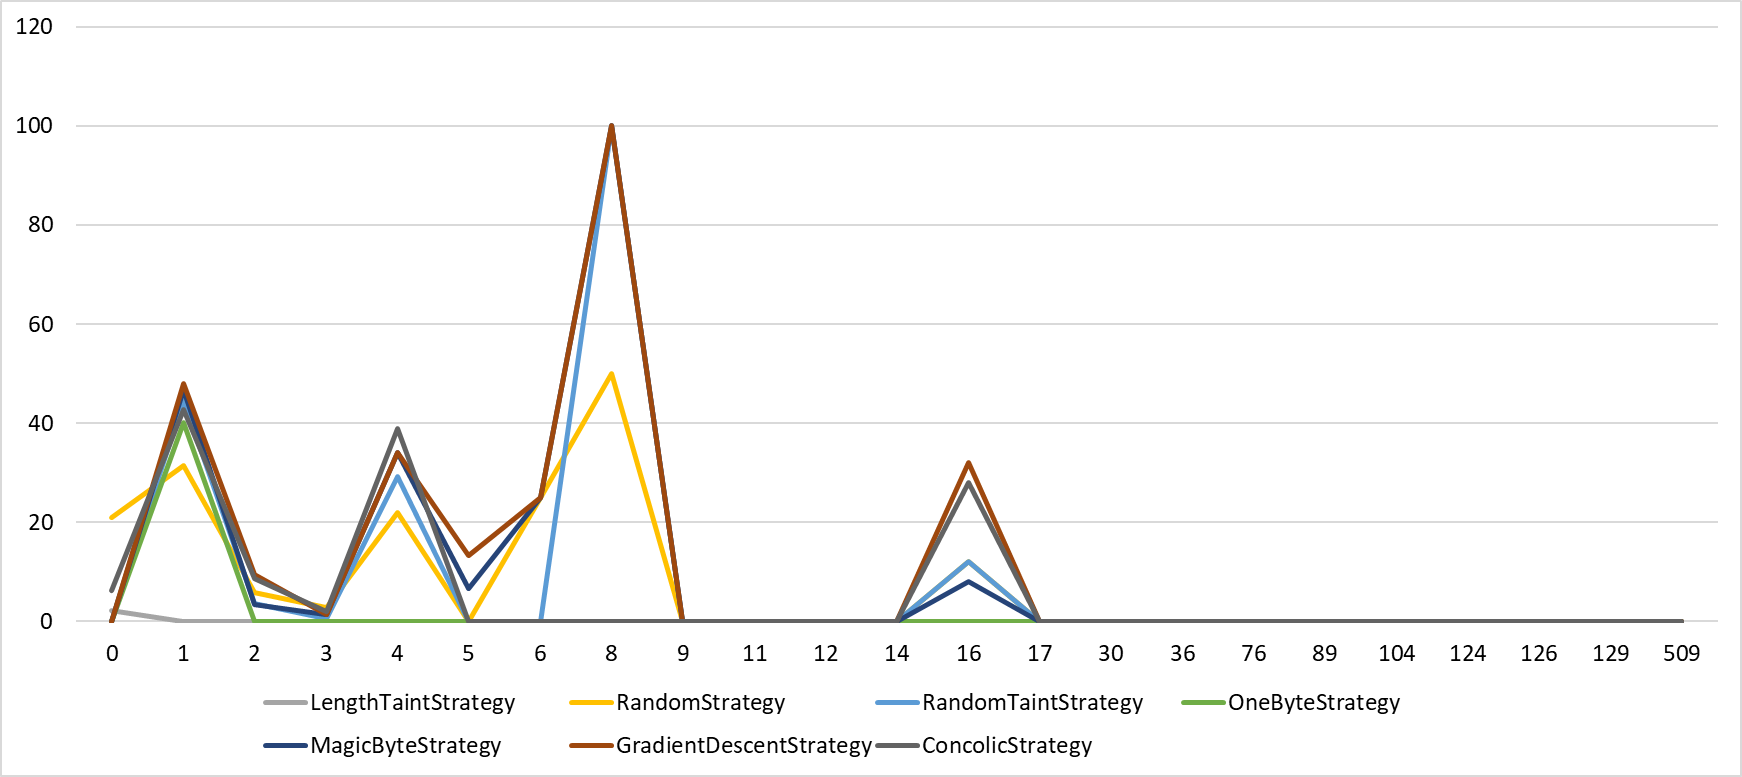
\includegraphics[width=.8\linewidth]{5_results/graphs/file-offsets.png}  
    \caption{Percentage of conditions flipped per number of offsets present from the input in the \texttt{file} binary.}
    \label{fig:fileOffsets}
\end{figure}

In the \texttt{file} program, we find that some condition exists, for which 509 offsets from the input were required to flip which can be seen in Figure \ref{fig:fileOffsets}. We see further peaks at some offsets, but no condition with more than 16 offsets were flipped.
\begin{figure}[H]
    \centering
    % include first image
    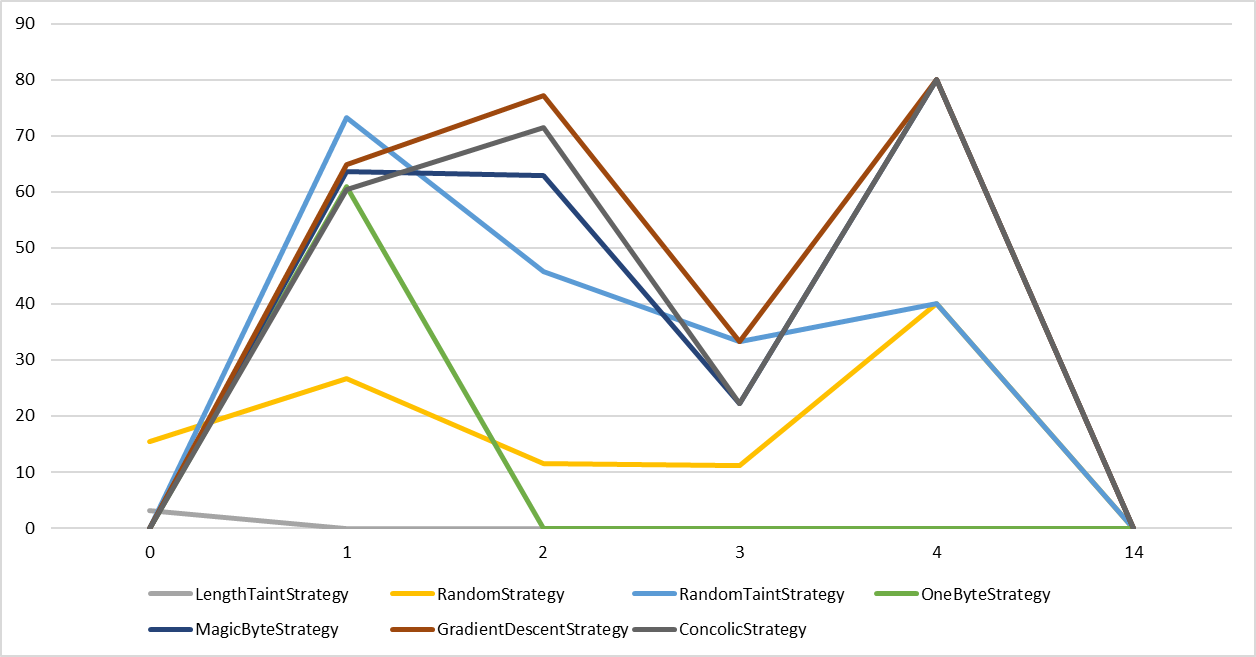
\includegraphics[width=.8\linewidth]{5_results/graphs/gif2png-offsets.png}  
    \caption{Percentage of conditions flipped per number of offsets present from the input in the \texttt{gif2png} binary.}
    \label{fig:gif2pngOffsets}
\end{figure}
Again we see that the RandomStrategy creates flips for conditions for which no offsets were found in Figure \ref{fig:gif2pngOffsets}. This further enhances the idea that some information is lost during the taint tracking. We see that the MagicByte strategy finds more flips than the GradientDescent strategy for only 1 offset, but less for the other offsets.
\begin{figure}[H]
    \centering
    % include first image
    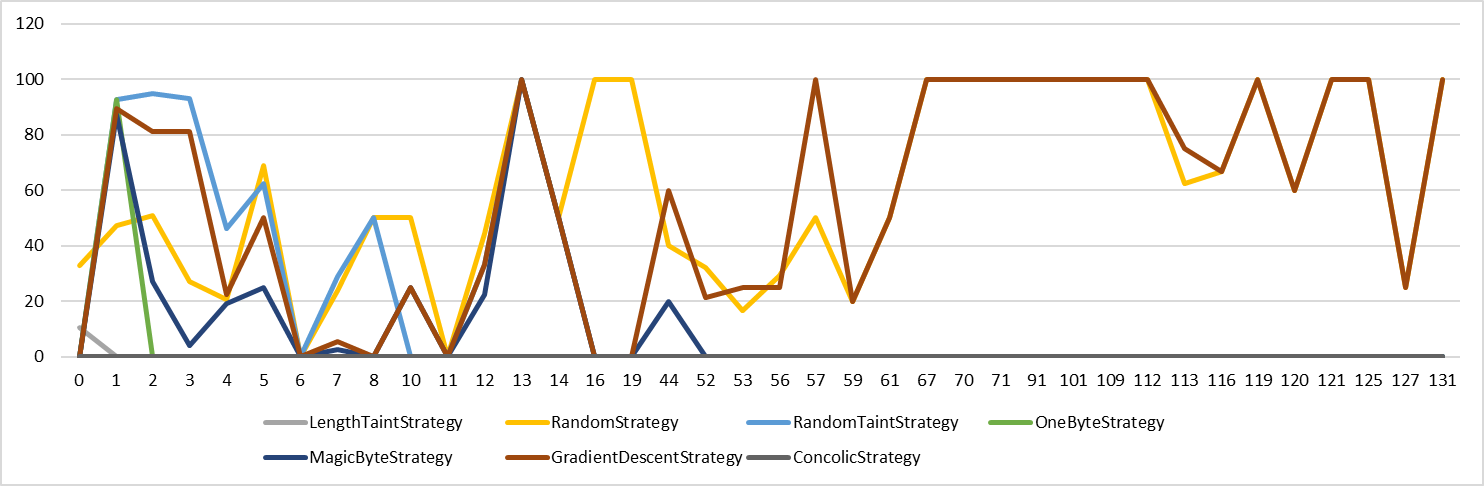
\includegraphics[width=.8\linewidth]{5_results/graphs/xmlwf-offsets.png}  
    \caption{Percentage of conditions flipped per number of offsets present from the input in the \texttt{xmlwf} binary.}
    \label{fig:xmlwfOffsets}
\end{figure}
We see in Figure \ref{fig:xmlwfOffsets} that even with a high number of offsets, the random strategy and GradientDescent strategy and RandomStrategy find flips for conditions with more than 100 offsets present in the input.
\begin{figure}[H]
    \centering
    % include first image
    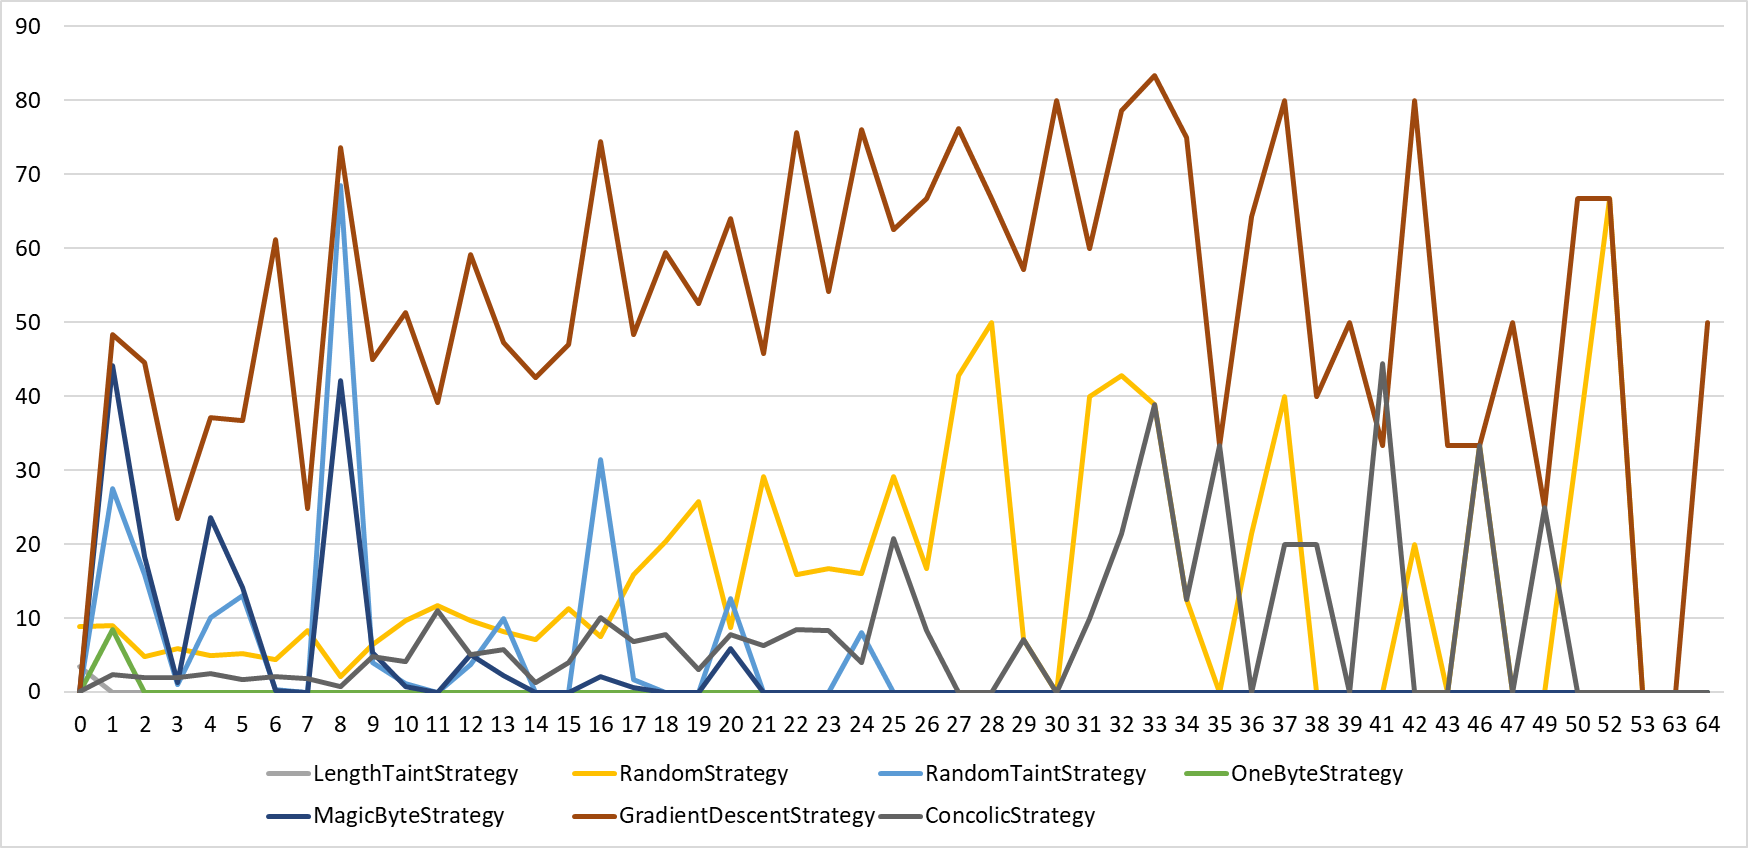
\includegraphics[width=.8\linewidth]{5_results/graphs/nm-offsets.png}  
    \caption{Percentage of conditions flipped per number of offsets present from the input in the \texttt{nm} binary.}
    \label{fig:nmOffsets}
\end{figure}
We see in Figure \ref{fig:nmOffsets} that the RandomTaintStrategy finds no flips for conditions with more than 25 offsets in the input, but the gradient descend and ConcolicStrategy do find flips for more flips. The RandomStrategy still finds flips which the RandomTaint strategy does not, which might indicate that we randomize too much in the RandomTaintStrategy.

From these graphs we get the idea that again the structure of the binary determines which strategy works better. This is because for the \texttt{xmlwf} and \texttt{nm} binary a lot of flips were found for conditions with a large number of offsets, but not for the \texttt{file} binary.




\subsection{Time}
In this section we will look at the time spend in a strategy.
Mostly because we want to know the effectiveness of the strategies. For this, we give the average of every strategy with the minimum and the maximum per binary. We expect the ConcolicStrategy to use a lot of time, but the other strategies way less.
The results are shown in Table \ref{appendix:timings} in seconds.
We notice that for the \texttt{file} binary, the ConcolicStrategy has ran for more than 10 seconds. After inspection, this could happen when a concolic run does not generate results, but the system call to terminate the process does not return immediately.
We indeed conclude that the ConcolicStrategy is several orders of magnitude slower than the other strategies for every binary. The MagicByte and OneByteStrategy only continue with the strategy if offsets are present, so the average gets influenced by the large number of executions where only a single check was performed.
This is also the case for the GradientDescentStrategy. Only for the runs of the \texttt{nm} binary, the Concolic execution is faster than expected. It is still unclear why this is the case. 
We further notice that the difference in speed between the Concolic and other strategies can be a factor 10 to 100 times faster on average. So symbolic execution should really be used as a last case resort if you want to preserve speed, which is also what \cite{stephens2016driller} and \cite{han2019synfuzz} use as approach to hybrid fuzzing.


